% Trajektorien-Punkte der Bahnplanung
% Author : Tobias Roth

\newcommand\Punkt{\tikz[scale=0.07]\draw[thick](-1,-1)--(1,1)(-1,1)--(1,-1);} 

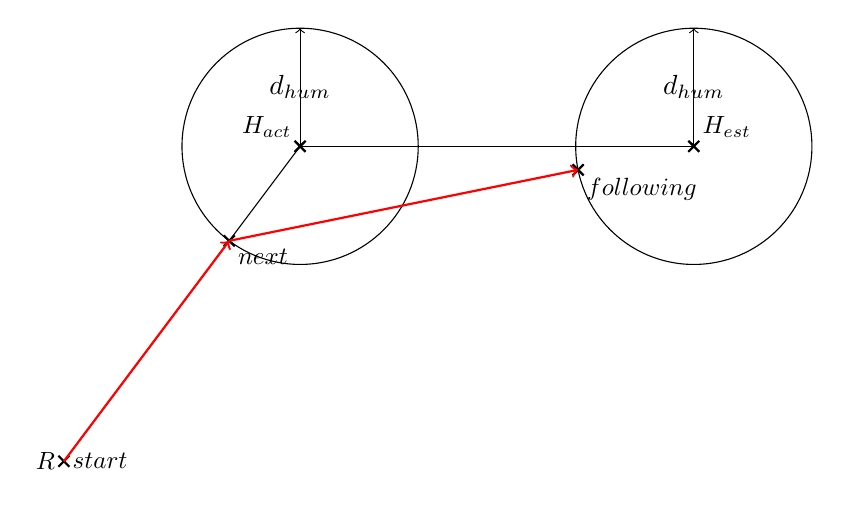
\begin{tikzpicture}


\def \dHum {1.5}

% Definition der Koordinaten für Roboter, Mensch_act und Mensch_est
\def \rX {0}
\def \rY {0}
\def \hActX {3}
\def \hActY {4}
\def \hEstX {8}
\def \hEstY {4}

% Setzen der Koordinaten für Roboter, Mensch_act und Mensch_est
\coordinate (r) at (\rX,\rY);
\coordinate (hact) at (\hActX,\hActY);
\coordinate (hest) at (\hEstX,\hEstY);

% Berechnung der Trajektorien-Punkte
\coordinate (trajPointA) at (r);
\coordinate (trajPointB) at (2.1, 2.8);	% hart codiert..
\coordinate (trajPointC) at (6.53095, 3.70137);	% hart codiert..

% Poitionen zeichnen
\node at (r) (R) {\Punkt};
\node[scale=0.9] at (r) [anchor=east] {$R$};
\node at (hact) (H_act) {\Punkt};
\node[scale=0.9] at (hact) [anchor=south east] {$H_{act}$};
\node at (hest) (H_est) {\Punkt};
\node[scale=0.9] at (hest) [anchor=south west] {$H_{est}$};

\node[scale=0.9] at (r) [anchor=west] {$start$};
\node at (trajPointB) (B) {\Punkt};
\node[scale=0.9] at (trajPointB) [anchor=north west] {$next$};
\node at (trajPointC) (C) {\Punkt};
\node[scale=0.9] at (trajPointC) [anchor=north west] {$following$};

% Vektoren zwischen Positionen
%\path[name path global=rHact, -] (r) edge (hact);
\path[-] (r) edge (hact);
\path[-] (hact) edge (hest);

% d_{Hum} zeichnen
%\draw [name path global=hactCircle] (hact) circle (\dHum);
%\draw [name path global=hestCircle] (hest) circle (\dHum);
\draw (hact) circle (\dHum);
\draw (hest) circle (\dHum);
\path[<->] (hact) edge node {$d_{hum}$} (\hActX,\hActY + \dHum);
\path[<->] (hest) edge node {$d_{hum}$} (\hEstX,\hEstY + \dHum);

% Eigentliche Trajektorie zeichnen
\path[red, thick, ->] (trajPointA) edge (trajPointB);
\path[red, thick, ->] (trajPointB) edge (trajPointC);



% Eigentliche Trajektorie zeichnen
% \path [name intersections={of=rHact and hactCircle, by={A}}];
% \node at (A) [below] {$A$};
% \path [name intersections={of=hactCircle and rHact}];
% \coordinate [label=above:$C$] (C) at (intersection-0);


\end{tikzpicture}
